Jako první určíme rozměry použitých tranzistoru.
Volím délku kanálu \(L = 2 [\mu m]\) jako kompromis mezi velikostí a parametrem \(\lambda\), která pro \(L = 2 \mu m\) nabývá hodnoty \(\lambda = 0.0787698 [V^{-1}]\).
Dále musíme zvolit napětí \(U_{OV}\), které volím \(U_{OV} = 0.5 [V]\) jelikož pracovní napětí mám jasně dané, větší pracovní rozsah tak nepotřebuji a radši použiji menší tranzistor.
Z toho následně můžeme určit šířku kanálu \(W\) jako:

\begin{center}
    \large
    \(
        W = L \cdot \frac{2 \cdot I_T}{KP \cdot U_{OV}^2} = 2\mu \cdot \frac{2 \cdot 40\mu}{200\mu 0.5^2} = 3.2 [\mu m]
    \)
\end{center}

Dále určíme společný odpor rezistorů \(r_2\) a \(r_3\) jako:

\begin{center}
    \large
    \(
        r_{2,3} = \frac{U_{OUT}}{I_1-I_2} = \frac{1.2}{50\mu - 50\mu} = 120 [k\Omega] 
    \)
\end{center}

Z čehož můžeme určit \(r_3\) jako:

\begin{center}
    \large
    \(
        r_3 = \frac{U_{TH}+U_{OV}}{U_{OUT}} \cdot r_{2,3} = \frac{0.384+0.5}{1.2} \cdot 120\cdot 10^{3} = 88.4 [k\Omega]
    \)
\end{center}

\(r_2\) pak určíme jednoduše jako:

\begin{center}
    \large
    \(
        r_2 = r_{2,3} - r_{3} = 120 \cdot 10^{3} - 88.4 \cdot 10^{3} = 31.6 [k\Omega]
    \)
\end{center}

Nakonec určíme odpor \(r_1\) jako:

\begin{center}
    \large
    \(
        r_1 = \frac{U_{CC}-U_{OUT}}{I_{1,2}} = \frac{1.8-1.2}{50\mu} = 12 [k\Omega] 
    \)
\end{center}

\vspace{10mm}
\begin{figure}[h!]
    \centering
    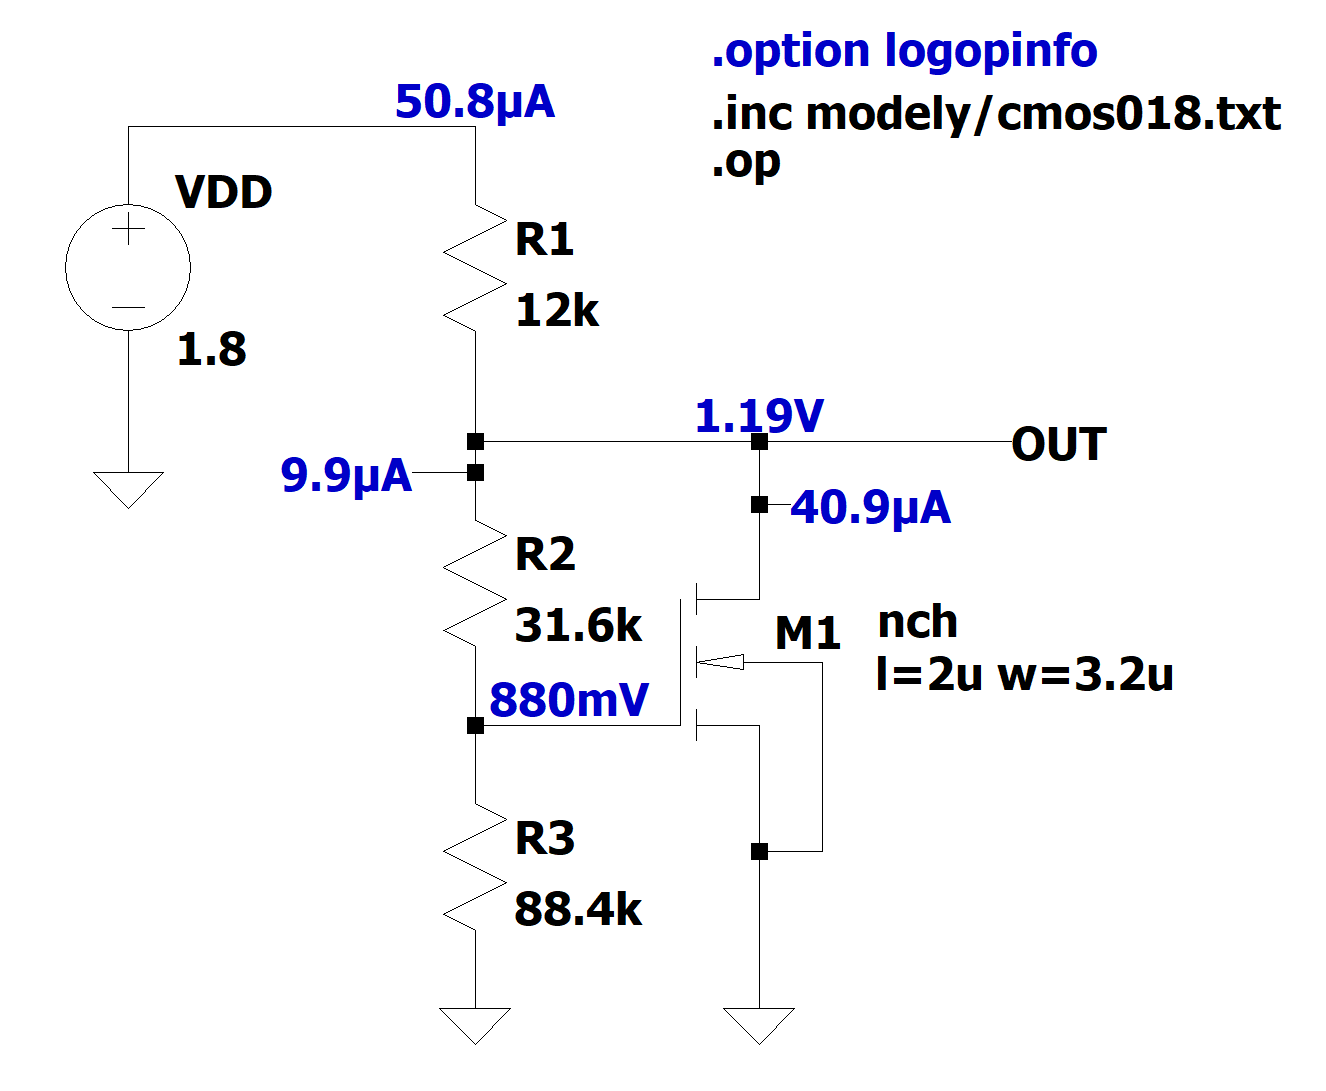
\includegraphics[width=0.9\textwidth]{text/img/NR-op-sch.png}
    \caption{\label{fig:NR-op-sch} Zobrazení napětí a proudu ve schématu}
\end{figure}

\vspace{10mm}
\begin{figure}[h!]
    \centering
    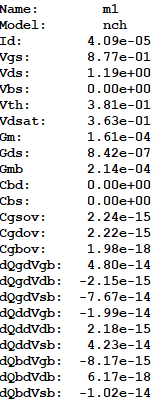
\includegraphics[width=0.3\textwidth]{text/img/NR-op-ol.png}
    \caption{\label{fig:NR-op-ol} Pracovní bod tranzistoru}
\end{figure}

